\documentclass[]{interact}

%\usepackage[caption=false]{subfig}% Support for small, `sub' figures and tables
%\usepackage[nolists,tablesfirst]{endfloat}% To `separate' figures and tables from text if required
%\usepackage[doublespacing]{setspace}% To produce a `double spaced' document if required
%\setlength\parindent{24pt}% To increase paragraph indentation when line spacing is doubled
%\setlength\bibindent{2em}% To increase hanging indent in bibliography when line spacing is doubled

\usepackage[numbers,sort&compress]{natbib}% Citation support using natbib.sty
\bibpunct[, ]{[}{]}{,}{n}{,}{,}% Citation support using natbib.sty
\renewcommand\bibfont{\fontsize{10}{12}\selectfont}% Bibliography support using natbib.sty

\usepackage{amsmath}
\usepackage{algorithm}
\usepackage{algpseudocode}
\usepackage[T1]{fontenc}
\usepackage{pgfplots}
\usetikzlibrary{arrows}
\pgfplotsset{compat=1.16}
\usepackage{caption}
\usepackage{subcaption}
\usepackage{minted}

\usepackage[hidelinks]{hyperref}

\theoremstyle{plain}% Theorem-like structures provided by amsthm.sty
\newtheorem{theorem}{Theorem}[section]
\newtheorem{lemma}[theorem]{Lemma}
\newtheorem{corollary}[theorem]{Corollary}
\newtheorem{proposition}[theorem]{Proposition}

\theoremstyle{definition}
\newtheorem{definition}[theorem]{Definition}
\newtheorem{example}[theorem]{Example}

\theoremstyle{remark}
\newtheorem{remark}{Remark}
\newtheorem{notation}{Notation}

\newcommand{\RR}{\mathbb{R}}
\newcommand{\norm}[2]{\left\| #1 \right\|_{#2}}
\newcommand{\abs}[1]{\left| #1 \right|}


\begin{document}

%\articletype{ARTICLE TEMPLATE}% Specify the article type or omit as appropriate

\title{Adaptive mesh refinement for locating free boundaries in obstacle problems}

\author{
\name{G.~Stefano Fochesatto\thanks{CONTACT G.~Stefano Fochesatto Email: gsfochesatto@alaska.edu} and Ed Bueler}
\affil{Dept.~of Mathematics and Statistics, University of Alaska Fairbanks, USA}
}

\maketitle

\begin{abstract}
Free-boundary problems posed as variational inequalities, such as obstacle problems, appear in scientific and engineering applications.  The geometrical error in the finite element (FE) solution of these problems, especially in locating the unknown free boundary and active/inactive sets, often dominates the overall numerical error.  In this paper we propose, and implement using the Firedrake FE library, adaptive mesh refinement (AMR) strategies which dynamically-enhance the mesh resolution around the free boundary.  These methods, which mark element for refinement based on a computed solution, reduce both geometrical and norm errors while controlling the growth of mesh complexity.  We consider three AMR methods: (i) an unstructured dilation operator based on discrete adjacency to the computed free-boundary; (ii) a variable-coefficient diffusion method which thresholds a diffused active set indicator function; and (iii) a metric-based method which averages an anisotropic, Hessian-derived Riemannian metric with an isotropic metric computed from the same diffused active set indicator.  The methods are evaluated by norm error decay, against mesh complexity and time, but geometric errors are also compared using Jaccard and Hausdorff distance methods.  Certain hybrid strategies are considered, combining these methods together, or with stages of uniform refinement.  Demonstrated applications include the classical Poisson obstacle problem and a shallow ice flow problem wherein one seeks a precise prediction of a glaciated region.
\end{abstract}

%\begin{keywords}
%FIXME
%\end{keywords}


\section{Introduction} \label{sec:intro}

The classical obstacle problem \cite{KinderlehrerStampacchia1980} finds the equilibrium position (vertical displacement) $u$ of an elastic membrane, attached to a fixed boundary, with some applied force $f$, but where the membrane is constrained to lie above some obstacle $\psi$.  Let $\Omega \subset \RR^d$ be a bounded domain, with the data $f$ and $\psi$ given on $\Omega$.  The strong formulation, a complementarity problem (CP), gives conditions satisfied by the solution $u$ almost everywhere in $\Omega$:
\begin{subequations} \label{eq:classical:ncp}
\begin{align}
  -\nabla^2 u - f \geq 0 \\
  u - \psi \geq 0\\
  (-\nabla^2u - f)(u - \psi) = 0
\end{align}
\end{subequations}
From a solution to \eqref{eq:classical:ncp} we may identify the inactive and active sets,
\begin{equation}
  I_u = \{x \in \Omega \,:\, u(x) > \psi(x)\}, \quad A_u = \Omega \setminus I_u, \label{eq:classical:sets}
\end{equation}
and the free boundary, which is where $I_u$ meets $A_u$ within $\Omega$:
\begin{equation}
  \Gamma_u = \Omega \cap \partial I_u. \label{eq:classical:free}
\end{equation}
From \eqref{eq:classical:ncp}, $u$ solves the Poisson equation $-\nabla^2u = f$ on $I_u$.  An example is shown in Figure \ref{fig:ball}, in which $A_u$ is the closed disc of contact ($u=\psi$), and $\Gamma_u$ is a circle.

\begin{figure}[H]
\centering
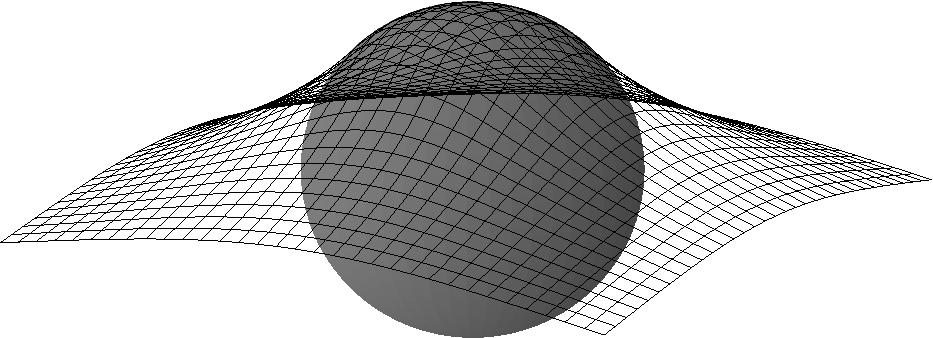
\includegraphics[width=0.7\textwidth]{static/obstacle65.pdf}
\caption{Solution $u$ of a classical obstacle problem; the obstacle $\psi$ is the upper hemisphere of a ball \cite[used by permission]{Bueler2021}.}
\label{fig:ball}
\end{figure}

As is well-known, such free-boundary problems have weak formulations which are variational inequalities (VIs) over Sobolev spaces.  Section \ref{sec:vifem} starts by stating this form.  In the case of the classical obstacle problem, and certain other cases, such VIs are equivalent to constrained minimization of a functional, but we will not need to consider that form, and for a later glacier example no such optimization form exists (Section \ref{sec:app}).

The finite element (FE) approximation of free-boundary problems necessitates such a VI form.  As in the case of PDEs \cite{ElmanSilvesterWathen2014}, if one describes both the exact solution $u$ by a VI, and its FE solution $u_h$, computed on some finite mesh with characteristic size $h>0$, then the norm errors $\|u-u_h\|$ can be computed in certain norms, and related to the approximation properties of the FE space.  For FE approximations of VIs there is a (now classical) framework for such \emph{a priori} norm error estimation \cite{Falk1974}; this theory is recalled in Section \ref{sec:vifem}.  Note that the current paper considers only meshs of triangles in dimension $d=2$, and one case with tetrahedra for $d=3$ (Section \ref{sec:results}), but VIs can be solved with higher-order elements as well \cite{KeithSurowiec2024}. 

However, a point that is weakly acknowledged, in the PDE-motivated FE literature for VIs \cite[for example]{Suttmeier2008}, regarding free-boundary problems, is that the geometrical mesh error in locating the free-boundary $\Gamma_u$ is, by itself, explanatory regarding the numerical error.  This situation is particularly clear in one dimension.  Consider, for example, the case where $\Omega = (-1,1)$ and the obstacle is a parabola, $\psi(x)=0.5 - x^2$.  With zero Dirichlet boundary conditions, the exact solution of the obstacle problem is easily calculated, with free boundaries at exact locations $x_*=\pm(2-\sqrt{2})/2$ (Figure \ref{fig:parabola}).  Now solve the FE approximation of this problem, using piecewise-linear elements and uniform meshes.  Since the exact free boundary is irrational, the mesh nodes will never coincide exactly.  Let $\Delta_h$ be defined as the minimum distance between the nodal coordinate and $x_*$, over a uniform mesh of elements of size $h$.  Figure \ref{fig:parabola} (right) shows the $H^1$ and $L^2$ norm errors $\|u-u_h\|$, computed in the usual manner, along with $\Delta_h$.  We see that the purely geometrical error $\Delta_h$, i.e.~the error in approximating $x_*$, and not other aspects of the error, fully explains the otherwise erratic behavior in norm errors.

\begin{figure}[H]

\mbox{
\begin{minipage}[t]{0.45\textwidth}
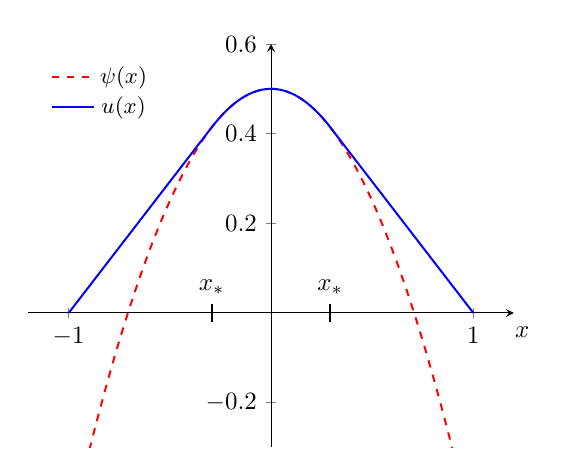
\begin{tikzpicture}[scale=0.9]
    \begin{axis}[
      axis lines = middle,
      xlabel = {$x$},
      xlabel style = {at={(1.05, 0.25)}},  % relative to whole figure box [0,1]x[0,1]
      domain = -1:1,
      samples = 100,
      xmin = -1.2,
      xmax = 1.2,
      ymin = -0.3,
      ymax = 0.6,
      xtick = {-1,1},
      legend pos = north west,
      legend style = {draw=none, font=\small}
    ]
      % Parameters
      \def\b{(2-sqrt(2))/2}
      \def\a{-\b}
      % Plot the obstacle function psi(x)
      \addplot[
        thick,
        red,
        dashed
      ] {0.5 - x^2};
      \addlegendentry{$\psi(x)$}
  
      % Plot u(x) in three pieces
      \addplot[
        thick,
        blue,
        domain=-1:\a
      ] {((.5 - \a*\a)/(\a + 1))*(x + 1)};
      \addplot[
        thick,
        blue,
        domain=\a:\b
      ] {0.5 - x^2};
      \addplot[
        thick,
        blue,
        domain=\b:1
      ] {-((.5 - \b*\b)/(1 - \b))*(x - 1)};
      \addlegendentry{$u(x)$}

      % indicate free boundary locations
      \addplot[black, thick, draw] coordinates {(\a,-0.02) (\a,0.02)} node[above] (A) {$x_*$};
      \addplot[black, thick, draw] coordinates {(\b,-0.02) (\b,0.02)} node[above] (B) {$x_*$};
    \end{axis}
  \end{tikzpicture}
  
\end{minipage}
\quad
\begin{minipage}[t]{0.55\textwidth}
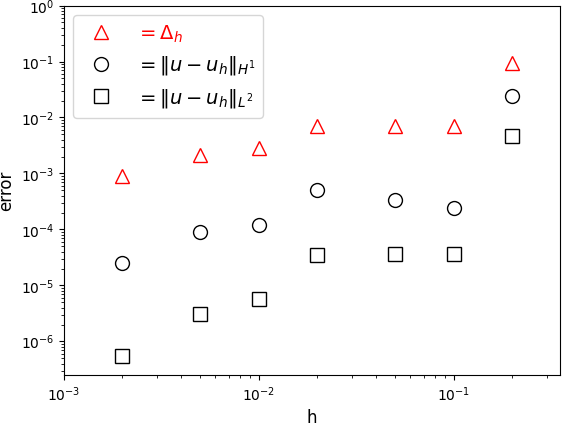
\includegraphics[width=0.9\textwidth]{static/VIConvergence.png}
% FIXME regenerate with labels ||u-u_h||_{H^1} = O(h^1.09), ||u-u_h||_{L^2} = O(h^1.57), \Delta_h
\end{minipage}
}
\caption{Left:  A one-dimensional obstacle problem with a parabolic obstacle, for which the exact free boundary locations $x_*$ are known.  Right:  Using uniform meshes, the geometrical error $\Delta_h$ in locating $x_*$ explains the erratic error norm $\|u-u_h\|$ behavior.}
\label{fig:parabola}
\end{figure}

FIXME of course more complicated when $d\ge 2$, but this justifies heuristic AMR just to pin down the free boundary, in addition to traditional VI AMR which will involve increasing the accuracy of $u_h$ over $I_h$

FIXME OLD STUFF FROM HERE The goal of this project is to introduce two techniques for adaptive mesh refinement for free boundary problems (variational inequalities).

In the context of the finite element method (FEM), the discretization of a partial differential equation (PDE) is described by a partition of its domain into a finite number of elements (i.e a mesh) and a finite dimensional function space (i.e a finite element space). In a two dimensional domain, these elements are usually triangles or rectangles and the basis of the finite element space is composed of hat functions over vertices in the mesh, with support over neighboring elements. 

The convergence of finite element solutions is most commonly achieved via approximating on increasingly refined meshes by the use of a finite basis of piecewise polynomials of low degree; this method of convergence is often referred to as $h$-refinement. We also see convergence achieved by approximating via increasingly higher degree basis of piecewise polynomials over a coarse mesh; this is referred to as $p$-refinement. Several schema have been explored that take advantage of both methods of convergence, so-called $hp$-refinement finite elements, further discussion of such methods can be found in \cite{Demkowicz2007}.

In terms of numerics, the constraint of $u \geq \psi$ makes this problem nonlinear so we are required to use an iterative solver. In this project our main solver will be VI-adapted Newton with Reduced-Space Line Search (VINEWTONRSLS). In Chapter 3 we will show that numerical methods will not converge until the active and inactive sets stabilize and the free boundary is identified. For solvers like VINEWTONRSLS which employ a Newton iteration, we find that they can only adjust the approximated free boundary by one-cell per iteration \citep{GraeserKornhuber2009} and therefore convergence is tied to mesh resolution and is proportional to the number of grid spaces between initial iterate free boundary and discrete solution free boundary \citep[page 324]{Bueler2021}. 

Adaptation involves altering the discretization to achieve a more desirable solution, whether that be with the goal of reducing $L_2$ error or reducing the error in some post-computation quantity like drag or lift. For example, consider the flow of some incompressable fluid through a pipe with an obstructive obstacle. Computing its drag coefficient would be an example of such a desired quantity \citep[Chapter 1.1]{BangerthRannacher2003}.

Further -adaptive methods have also been explored. These methods are designed to increase mesh resolution or polynomial degree locally by means of a local error estimator, for some goal term often referred to as the Quantity of Interest (QoI), and is also usually denoted as $J(\cdot)$. The most common of these employ the Dual Weighted Residual (DWR) method, derived in \cite{RannacherSuttmeier1997}. The DWR method, like most adaptive refinement techniques begins with a rigorous, a posteriori or a priori analysis of the quantity $J(u) - J(u_n)$. Estimation of this error quantity is then decomposed into local element-wise error estimators which can be used as a heuristic to tag elements for refinement. Finally a refinement strategy is employed to refine the mesh. Choices of whether to refine elements or increase the degree of polynomial basis functions, and by how much, must be made. 

The techniques outlined above are referred to as tagging methods, in which the error indicators are used to 'tag' elements for refinement. However, there are 'metric-based' methods which control the size, shape and orientation of the elements instead \citep{Alauzet2010}.  For this project we will primarily focus on $h$-adaptive tagging methods.

As we will see in Chapter 3, convergence of VI problems is dominated by the error in approximating the free boundary. An adaptive refinement scheme that is able to concentrate effort around the solution free boundary will both, enhance convergence properties and reduce unnecessary computation in the active set.


In this project we will introduce two adaptive refinement schemes which can identify the free boundary to a high degree of accuracy and permit the user to vary the spread of the refinement area. In the first strategy we compute a node-wise indicator function for the active set for use as an initial iterate in a single step of a time-dependent heat equation problem. Solving a single step of this problem has the effect of smoothing the indicator about the free boundary. The result of this smoothing is then averaged over each element and thresholded for refinement.  The second strategy focuses on the discrete identification of elements adjacent to the free boundary, employing a graph-based approach to mark neighboring elements for refinement.  This generalizes the bitmap image processing operation of dilation [cite] to unstructured meshes.

Our implementations of these methods are written using the Firedrake finite element library and produce conforming meshes with no hanging nodes. These high quality meshes are suitable for various VI solvers, including as coarse grids for the FASCD multilevel solver in \cite{BuelerFarrell2024}

FIXME The remaining material is organized as follows.  We give a brief background on solving VIs numerically.  Via a 1D example, we illustrate why the error arising from the geometric error in approximating the free boundary dominates the overall numerical error.   Then we introduce the two new adaptive refinement schemes for VIs, VCES and UDO, and provide a detailed description of their implementations.  The results section demonstrates the effectiveness of the proposed methods in enhancing mesh resolution around free boundaries. 


\section{Variational inequalities and their finite element errors} \label{sec:vifem}

We seek to find the position of the membrane $u(x)$, with fixed valued $u(x) = g_D(x)$ on $\partial \Omega$ with a load $f$ applied, and where $u(x)$ is constrained to be above an obstacle $\psi(x)$, 
The admissable set for such a problem can be described by 
  \begin{equation}
    K_\psi = \{u \in X| u \geq \psi \}
  \end{equation}
  where $X$ is a Sobolev space with boundary conditions $g_D$ enforced. 
  
  We can describe another, equivalent, variational inequality (VI) formulation of the obstacle problem 
  \begin{equation}
    \int_\Omega \nabla u \cdot \nabla(v - u) \geq \int_\Omega f(v - u), \quad \text{ for all } v \in K_\psi.
  \end{equation} 
Sets $I_u$, $A_u$, and $\Gamma_u$ are defined in the Introduction.

FIXME Cea's lemma and Falk technique

%FIXME \cite{ElmanSilvesterWathen2014} \cite{Suttmeier2008}
%FIXME \cite{Kosub2016} \cite{JungeblutKleistMiltzow2022}


\section{New adaptive mesh refinement strategies} \label{sec:viamr}

To explain our methods for adaptive mesh refinement for VIs, we will first review certain methods for adaptive mesh refinement from the literature for PDEs.  Tagging methods, are a class of adaptive methods which assess the suitability of a mesh element-by-element in computing a Quantity of Interest (QoI) like $L_2$ error or another post computation functional like drag or lift \cite{bangerth_adaptive_2003}. The main idea behind most tagging methods is the refinement loop:

\begin{algorithm}
  \caption{Tag and refine}
  \begin{algorithmic}
    \State Solve: Solve the PDE on the current mesh. 
    \State Estimate: Estimate the error in the QoI element-by-element.
    \State Tag: Tag elements for refinement based on the error estimate.
    \State Refine: Refine or coarsen the mesh maintaining the minimum angle criteria.
  \end{algorithmic}
\end{algorithm}

Throughout the literature (\citet{becker_feed-back_1996}, \citet{bangerth_adaptive_2003}, \citet{suttmeier_numerical_2008}) one finds a variety of ways to perform the "Estimate" step. As we mentioned in the Introduction a common way is by the Dual Weighted Residual (DWR) method introduced in \citet{becker_feed-back_1996}. For further details see \citet[Chapter 3]{bangerth_adaptive_2003}. A general approach for extending the DWR method to variational inequalities can be found in \citet{suttmeier_numerical_2008}.  However, the methods proposed here are not based on the DWR method. 

There are also several ways to perform the "Tag" step. Consider the following fixed-rate strategy found in \citet[Chapter 4]{bangerth_adaptive_2003}. For fractions $X, Y$ with $1 - X > Y$ and a mesh with $N$ elements, refine the $X\cdot N$ elements with the largest error indicator and coarsen the $Y\cdot N$ elements with the smallest error indicator. For appropriate choices of $X$ and $Y$ this has the effect of keeping the degrees of freedom almost constant. There are other more exotic solutions which accomplish different goals. For example there is a fairly impractical "error-balancing" strategy also described in \citet[Chapter 4]{bangerth_adaptive_2003} which seeks to equilibrate the error indicators across the mesh.

The "Refine" step in Algorithm 2 addresses to refine cells once they have been selected for refinement. This process involves two considerations: maintaining the minimum angle condition and managing hanging nodes. As illustrated in Figure 2.4, elements can be refined in such a way that the minimum angle condition is violated, leading to poor convergence properties. The second issue concerns hanging nodes, which are nodes that do not have a "covering" relation to all neighboring elements; this concept will be elaborated on further.

A tagging strategy like the one above can be implemented in Firedrake using Netgen/NGSolve integration \citep{zerbinati_ngspetsc_nodate}.  This integration brings several new features to Firedrake, but for our purposes the most important is the \texttt{refine\_marked\_elements()} method.  This method resides inside of a netgen mesh object and takes an indicator function over the domain representing which elements are marked for refinement. This method is capable of dealing with hanging nodes by use of transition cells

The operation of interpolating a function into a DG0 space is central to our proposed methods for adaptive refinement. Conceptually this operation allows us to compute estimators (Estimate step of Algorithim 2) which take on a single value over vertices and then convert them, by averaging over an element into an estimator which takes on a single value over the element. Averaging a function over elements is equivalent to interpolation into a DG0 space. To see this, consider the definition of the interpolation operation given in the Firedrake user manual \citep{ham_firedrake_2023}. 
Let $u$ be a function over some domain $\Omega$ and $V$ be a finite element space defined on $\Omega$ with basis $\{\phi_i\}_{i = 1}^N$. Then $interpolate(u, V)$ is given by $\sum_{i = 1}^N v_i \phi_i$ where $v_i = \phi^*_i$ and $\phi^*_i$ is an element of the dual basis of $V$. (Recall that the dual basis of $V_\Omega$ is given by the vector $\{\phi^*_i\}$, such that $\phi^*_i(\phi_j) = \delta_{ij}$). The corresponding dual basis vector of a DG0 space is the following average
\begin{equation}
  \phi_j^*(f) = \frac{1}{area(\triangle_j)}\int_{\triangle_j} f\, dx.
\end{equation}
Note that this choice of functional has the property that $\phi^*_i(\phi_j) = \delta_{ij}$. Now $interpolate(u, V) = \sum_{i = 1}^n v_i\theta_i$ where
\begin{equation}
  v_i = \frac{1}{area(\triangle_i)}\int_{\triangle_i} u \, dx.
\end{equation}

We propose two strategies for adaptive refinement of variational inequalities, which we call Variable Coefficient Elliptic Smoothing (VCES) and Unstructured Dilation Operator (UDO). These methods are designed to enhance mesh resolution at the free boundary found when solving the VI. These methods are the Estimate and Tag steps in Algorithm 2. They effectively control the error associated with approximating the free boundary, as observed in Section 3.3 and illustrated in Figure 3.4. Note that Firedrake/Netgen is used for the Solve and Refine steps in Algorithim 2.

The first strategy is called Variable Coefficient Elliptic Smoothing (VCES). The idea is to use the residual $u^k - \psi$ and a positive tolerance to construct $s_0$, a node-wise indicator function for the active set. This indicator function is used as the initial condition of a variable-coefficient and time-dependent heat equation problem which has the effect of smoothing this indicator near the free boundary. This heat equation problem is solved for a single timestep via implicit Euler, the result of which, we'll call $s_1$. This problem is a linear elliptic PDE, hence "elliptic smoothing"
\begin{equation}
  \frac{1}{\Delta t}(s_1 - s_0) = \nabla^2 s_1.
\end{equation}
Our choice of timestep $\Delta t_i = \frac{1}{2}(\text{avg}(\text{diam}(\triangle_i)))^2$ where $\triangle_i$ is the set of all elements incident to vertex $i$. This choice depends on the element, thus "variable coefficient". Varying the timestep based off of neighboring element diameter has the effect of applying the same amount diffusion across all elements regardless of size. The result is then interpolated into a DG0 space and thresholded to produce the refinement indicator, as in Algorithim 2. There are various parameters to consider with this technique. The choice of timestep and thresholding parameters will substantially affect the "distance" about which the free boundary is resolved. 

\begin{algorithm}[H]
	\caption{Variable Coefficient Elliptic Smoothing Element Tagging for VIs}\label{alg:cap}
	\begin{algorithmic}[1]
		\Require $tol \in \mathbb{R}$, $u^k \in K_\psi, \psi \in V$, $W$ is DG0 FE space.
		\Require Threshold parameters $0\leq \alpha < \beta \leq 1$.
		\State Compute the nodal active set indicator function $s_0$
		  \begin{equation*}
			s_0 = \begin{cases}
			  1 & \text{ if } u^k - \psi < tol\\
			  0 & \text{ otherwise}
			\end{cases}
		  \end{equation*}
		\State Let $\Delta t_i = \frac{1}{2}(\text{avg}(\text{diam}(\triangle_i)))^2$, a CG1 field.
	  
		\State Solve $\frac{1}{\Delta t}(s_1 - s_0) = \nabla^2 s_1$ with $g_D = s_0|_{\partial\Omega}$ impliclty with Firedrake defaults settings. 
		\State Let $s_W = interpolate(s_1, W)$.
		\State Define the refinement indicator $I \in W$ as follows:
		\begin{equation*}
		  I(\triangle) = \begin{cases}
			1 & \text{ if } \alpha < s_W(\triangle) < \beta\\
			0 & \text{ otherwise}
		  \end{cases}
		\end{equation*}\\
		\Return $I$
	\end{algorithmic}
	\end{algorithm}

Figure 5.1 illustrates the VCES algorithm applied to a one-dimensional obstacle problem.

\begin{figure}[H]
  \captionsetup[subfigure]{justification=centering}
  \centering
  \null\hfill
  \begin{subfigure}[b]{.35\textwidth}
    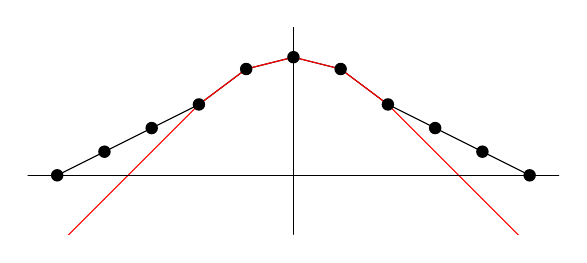
\begin{tikzpicture}[line cap=round,line join=round,>=triangle 45,scale=1.5]
      \clip(-2.25,-0.5) rectangle (2.25,1.25);
      \draw (0.4,0.9) -- (0.8,0.6);
      \draw (0.8,0.6) -- (1.2,0.4);
      \draw (1.2,0.4) -- (1.6,0.2);
      \draw (-0.4,0.9) -- (-0.8,0.6);
      \draw (-0.8,0.6) -- (-1.2,0.4);
      \draw (-1.2,0.4) -- (-1.6,0.2);
      \draw (-1.6,0.2) -- (-2,0);
      \draw (1.6,0.2) -- (2,0);
      \draw (-0.4,0.9) -- (0,1);
      \draw (0,1) -- (0.4,0.9);

      % New red curve aligning with black nodes
      \draw[red] (1.6,-.2) -- (2,-.6);
      \draw[red] (1.2,0.2) -- (1.6,-.2);
      \draw[red] (0.8,0.6) -- (1.2,0.2);
      \draw[red] (0.4,0.9) -- (0.8,0.6);
      \draw[red] (0,1) -- (0.4,0.9);
      \draw[red] (-0.4,0.9) -- (0,1);
      \draw[red] (-0.4,0.9) -- (-0.8,0.6);
      \draw[red] (-0.8,0.6) -- (-1.2,.2);
      \draw[red] (-1.2, .2) -- (-1.6,-.2);
      \draw[red] (-1.6,-.2) -- (-2,-.6);

      \begin{scriptsize}
        \fill [color=black] (-0.4,0.9) circle (1.5pt);
        \fill [color=black] (0.4,0.9) circle (1.5pt);
        \fill [color=black] (0.8,0.6) circle (1.5pt);
        \fill [color=black] (1.2,0.4) circle (1.5pt);
        \fill [color=black] (1.6,0.2) circle (1.5pt);
        \fill [color=black] (-0.8,0.6) circle (1.5pt);
        \fill [color=black] (-1.2,0.4) circle (1.5pt);
        \fill [color=black] (-1.6,0.2) circle (1.5pt);
        \fill [color=black] (-2,0) circle (1.5pt);
        \fill [color=black] (2,0) circle (1.5pt);
        \fill [color=black] (0,1) circle (1.5pt);
      \end{scriptsize}

      % Add Axes
      \draw[-] (-2.5,0) -- (2.5,0); % x-axis
      \draw[-] (0,-0.5) -- (0,1.45); % y-axis
    \end{tikzpicture}
    \caption{Iterate $u^k$(black) and obstacle $\psi$(red).}
  \end{subfigure}
  \hfill
  \begin{subfigure}[b]{.35\textwidth}
    \begin{tikzpicture}[line cap=round,line join=round,>=triangle 45,scale=1.5]
      \clip(-2.25,-0.5) rectangle (2.25,1.25);
      \draw (1.6,0) -- (2,0);
      \draw (1.2,0) -- (1.6,0);
      \draw (0.8,1) -- (1.2,0);
      \draw (0.4,1) -- (0.8,1);
      \draw (0,1) -- (0.4,1);
      \draw (-0.4,1) -- (0,1);
      \draw (-0.4,1) -- (-0.8,1);
      \draw (-0.8,1) -- (-1.2,0);
      \draw (-1.2,0) -- (-1.6,0);
      \draw (-1.6,0) -- (-2,0);

      % Add black vertices
      \begin{scriptsize}
        \fill [color=black] (1.6,0) circle (1.5pt);
        \fill [color=black] (2,0) circle (1.5pt);
        \fill [color=black] (1.2,0) circle (1.5pt);
        \fill [color=black] (0.8,1) circle (1.5pt);
        \fill [color=black] (1.2,0) circle (1.5pt);
        \fill [color=black] (0.4,1) circle (1.5pt);
        \fill [color=black] (0.8,1) circle (1.5pt);
        \fill [color=black] (0,1) circle (1.5pt);
        \fill [color=black] (0.4,1) circle (1.5pt);
        \fill [color=black] (-0.4,1) circle (1.5pt);
        \fill [color=black] (0,1) circle (1.5pt);
        \fill [color=black] (-0.4,1) circle (1.5pt);
        \fill [color=black] (-0.8,1) circle (1.5pt);
        \fill [color=black] (-1.2,0) circle (1.5pt);
        \fill [color=black] (-1.6,0) circle (1.5pt);
        \fill [color=black] (-2,0) circle (1.5pt);
      \end{scriptsize}
      
      % Add Axes
      \draw[-] (-2.5,0) -- (2.5,0); % x-axis
      \draw[-] (0,-0.5) -- (0,1.45); % y-axis
  
      % Label y=1
      \node at (-0.1,1.15) [left] {1};
      \draw[dashed] (-0.1,1) -- (0,1);
    \end{tikzpicture}
    \caption{Nodal active set indicator $s_0$.}
  \end{subfigure}
  \null\hfill
  \medskip

  \null\hfill
  \begin{subfigure}[b]{.35\textwidth}
    \centering
    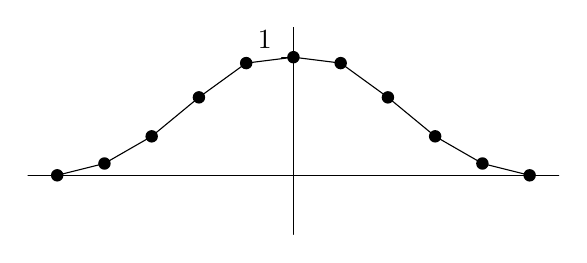
\begin{tikzpicture}[line cap=round,line join=round,>=triangle 45,scale=1.5]
      \clip(-2.25,-0.5) rectangle (2.25,1.25);
      
      % Draw the smoothed curve
      \draw (1.6, 0.1) -- (2,0);      
      \draw (1.2, 0.33) -- (1.6, 0.1);
      \draw (0.8, 0.66) -- (1.2, 0.33);
      \draw (0.4, 0.95) -- (0.8, 0.66);
      \draw (0,1) -- (0.4, 0.95);
      \draw (-0.4, 0.95) -- (0,1);
      \draw (-0.4, 0.95) -- (-0.8, 0.66);
      \draw (-0.8, 0.66) -- (-1.2, 0.33);
      \draw (-1.2, 0.33) -- (-1.6, 0.1);
      \draw (-1.6, 0.1) -- (-2,0);
  
      % Add black vertices
      \begin{scriptsize}
        \fill [color=black] (1.6, 0.1) circle (1.5pt);
        \fill [color=black] (2,0) circle (1.5pt);
        \fill [color=black] (1.2, 0.33) circle (1.5pt);
        \fill [color=black] (0.8, 0.66) circle (1.5pt);
        \fill [color=black] (0.4, 0.95) circle (1.5pt);
        \fill [color=black] (0,1) circle (1.5pt);
        \fill [color=black] (-0.4, 0.95) circle (1.5pt);
        \fill [color=black] (-0.8, 0.66) circle (1.5pt);
        \fill [color=black] (-1.2, 0.33) circle (1.5pt);
        \fill [color=black] (-1.6, 0.1) circle (1.5pt);
        \fill [color=black] (-2,0) circle (1.5pt);
      \end{scriptsize}
  
      % Add Axes
      \draw[-] (-2.5,0) -- (2.5,0); % x-axis
      \draw[-] (0,-0.5) -- (0,1.45); % y-axis
  
      % Label y=1
      \node at (-0.1,1.15) [left] {1};
      \draw[dashed] (-0.1,1) -- (0,1);
    \end{tikzpicture}
    \caption{Smoothed $s_1$.}
  \end{subfigure}
  \hfill
  \begin{subfigure}[b]{.35\textwidth}
    \centering
    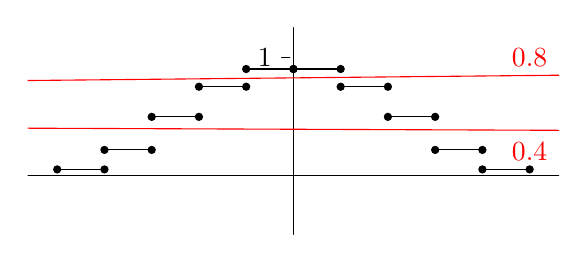
\begin{tikzpicture}[line cap=round,line join=round,>=triangle 45,scale=1.5]
      \clip(-2.25,-0.5) rectangle (2.25,1.25);

      % Draw horizontal segments at the heights of the calculated midpoints
      \draw (-2, 0.05) -- (-1.6, 0.05);
      \draw (-1.6, 0.215) -- (-1.2, 0.215);
      \draw (-1.2, 0.495) -- (-0.8, 0.495);
      \draw (-0.8, 0.75) -- (-0.4, 0.75);
      \draw (-0.4, 0.9) -- (0, 0.9);
      \draw (0, 0.9) -- (0.4, 0.9);
      \draw (0.4, 0.75) -- (0.8, 0.75);
      \draw (0.8, 0.495) -- (1.2, 0.495);
      \draw (1.2, 0.215) -- (1.6, 0.215);
      \draw (1.6, 0.05) -- (2, 0.05);

      % Add black vertices
      \begin{scriptsize}
        \fill [color=black] (-2, 0.05) circle (1pt);
        \fill [color=black] (-1.6, 0.05) circle (1pt);
        \fill [color=black] (-1.6, 0.215) circle (1pt);
        \fill [color=black] (-1.2, 0.215) circle (1pt);
        \fill [color=black] (-1.2, 0.495) circle (1pt);
        \fill [color=black] (-0.8, 0.495) circle (1pt);
        \fill [color=black] (-0.8, 0.75) circle (1pt);
        \fill [color=black] (-0.4, 0.75) circle (1pt);
        \fill [color=black] (-0.4, 0.9) circle (1pt);
        \fill [color=black] (0, 0.9) circle (1pt);
        \fill [color=black] (0, 0.9) circle (1pt);
        \fill [color=black] (0.4, 0.9) circle (1pt);
        \fill [color=black] (0.4, 0.75) circle (1pt);
        \fill [color=black] (0.8, 0.75) circle (1pt);
        \fill [color=black] (0.8, 0.495) circle (1pt);
        \fill [color=black] (1.2, 0.495) circle (1pt);
        \fill [color=black] (1.2, 0.215) circle (1pt);
        \fill [color=black] (1.6, 0.215) circle (1pt);
        \fill [color=black] (1.6, 0.05) circle (1pt);
        \fill [color=black] (2, 0.05) circle (1pt);
      \end{scriptsize}

      % Add Axes
      \draw[-] (-2.5,0) -- (2.5,0); % x-axis
      \draw[-] (0,-0.5) -- (0,1.25); % y-axis

      % Label y=1
      \node at (-0.1, 1) [left] {1};
      \draw[dashed] (-0.1, 1) -- (0, 1);

      % Add red horizontal lines at heights 0.8 and 0.4
      \draw[red] (-2.5, 0.8) -- (2.5, 0.85); % red line at y = 0.8
      \draw[red] (-2.5, 0.4) -- (2.5, 0.38);  % red line at y = 0.4
      % Label the heights of the red lines
      \node[red] at (2, 1) {0.8};
      \node[red] at (2, 0.2) {0.4};
    \end{tikzpicture}
    \caption{$interpolate(s_1,W)$. Threshold values in red.}
  \end{subfigure}
  \null\hfill
  \medskip

  \begin{subfigure}[b]{0.9\textwidth}
    \centering
    \begin{tikzpicture}[line cap=round,line join=round,>=triangle 45,scale=1.5]
      \clip(-2.5,-0.5) rectangle (2.5,1.25);
      
      \draw (1.6,0) -- (2,0);      
      \draw (1.2,0) -- (1.6,0);
      \draw (0.8,1) -- (1.2,1);
      \draw (0.4,1) -- (0.8,1);
      \draw (0,0) -- (0.4,0);
      \draw (-0.4,0) -- (0,0);
      \draw (-0.4,1) -- (-0.8,1);
      \draw (-0.8,1) -- (-1.2,1);
      \draw (-1.2,0) -- (-1.6,0);
      \draw (-1.6,0) -- (-2,0);
  
      % Add Axes
      \draw[-] (-2.5,0) -- (2.5,0); % x-axis
      \draw[-] (0,-0.5) -- (0,1.45); % y-axis
  
      % Label y=1
      \node at (-0.1, 1) [left] {1};
      \draw (-0.1, 1) -- (0, 1);
  
      % Add Nodes
      \begin{scriptsize}
      \fill [color=black] (1.6,0) circle (1.5pt);
      \fill [color=black] (2,0) circle (1.5pt);      
      \fill [color=black] (1.2,0) circle (1.5pt);
      \fill [color=black] (0.8,1) circle (1.5pt);
      \fill [color=black] (1.2,1) circle (1.5pt);
      \fill [color=black] (0.4,1) circle (1.5pt);
      \fill [color=black] (0.8,1) circle (1.5pt);
      \fill [color=black] (0,0) circle (1.5pt);
      \fill [color=black] (0.4,0) circle (1.5pt);
      \fill [color=black] (-0.4,0) circle (1.5pt);
      \fill [color=black] (0,0) circle (1.5pt);
      \fill [color=black] (-0.4,1) circle (1.5pt);
      \fill [color=black] (-0.8,1) circle (1.5pt);
      \fill [color=black] (-1.2,1) circle (1.5pt);
      \fill [color=black] (-1.2,0) circle (1.5pt);
      \fill [color=black] (-1.6,0) circle (1.5pt);
      \fill [color=black] (-2,0) circle (1.5pt);
      \end{scriptsize}
    \end{tikzpicture}
    \caption{Refinement indicator function $I$.}
  \end{subfigure}
  \vspace*{.25cm}
  \caption{Illustration of Variable Coefficient Elliptic Smoothing algorithm.}
\end{figure}

Support for unstructured meshes in Firedrake comes from the DMPlex class in PETSc, as developed by \citet{lange_flexible_2015}. DMPlex is a data management object which can store the topology (connectivity of mesh entities) and geometry (coordinates) of a discretization. In the DMPlex object every mesh entity is assigned a unique index. The connectivity of a mesh is stored as a layered directed acyclic graph (DAG) in which a "covering" relation specifies the edges of the graph. For example, for a tetrahedral element in a 3d mesh, a face is covered by 3 edges and a tetrahedral cell is covered by 4 faces. Each layer represents a class of mesh entity i.e vertices, edges, etc. Below is an example of how a single tetrahedral cell is represented by DMPlex.

The DMPlex object has several methods which make querying the mesh topology and geometry simple \citep{lange_efficient_2016}. For example, let $p$ be an index assigned by DMPlex. Then $\emph{cone}(p)$ returns all the in-neighbors of $p$. In the example above $\emph{cone}(0) = \{11, 12, 13, 14\}$. The transitive closure of $\emph{cone}(p)$ is also available with $\emph{closure}(p)$. The dual of $\emph{cone}(p)$ is $\emph{support}(p)$ which returns all the out-neighbors of $p$. In the example above $\emph{support}(6) = \{6, 7, 10\}$. The transitive closure of $\emph{support}(p)$ is also available with $\emph{star}(p)$. 

The use of DMPlex queries is essential to our second strategy, the Unstructured Dilation Operator (UDO). We identify the set $B$ of elements that border the computed free boundary $\Gamma_{u^k}$ by interpolating a nodal active indicator function into DG0 and thresholding for values in the range (0, 1). We then use the \emph{closure} and \emph{star} methods to create vertex-to-cell and cell-to-vertex mappings. These mappings are then used to determine which elements are neighbors to the computed free boundary. We say an element neighbors another if it shares at least one vertex. The function $N(\triangle)$ returns a set of elements:
\begin{equation}
  N(\triangle) = \{\triangle_i \in T: \triangle \text{ shares at least 1 vertex with } \triangle_i\}.
\end{equation}
This process is then repeated $n$ times to create a set of elements that are within $n$ neighborhood levels of the border elements:
\begin{equation}
  N^n(\triangle) = \underbrace{N(...N(\triangle))}_{n \text{ times}}.
\end{equation}
As show in Algorithim 3, for a border element set $B$, defined below in (5.5) we use breadth-first search to construct the set $N^n(B)$ and then assemble its corresponding indicator function. This process expand the support of the DG0 indicator function in a way that resembles the "dilation" operation in image processing as seen in \citep{OpenCV} but it is applied over an unstructured mesh.

\begin{algorithm}[H]
  \caption{Unstructured Dilation Operator Element Tagging for VIs}
  \begin{algorithmic}[1]
    \Require $tol \in \mathbb{R}$, $u^k \in K, \psi \in V$, $W$ is a DGO FE space, mesh $T$.
    \Require Neighborhood Depth Parameter $n \in \mathbb{N}$.
    \State Compute the nodal active set indicator function $s$
    \begin{equation}
    s = \begin{cases}
      1 & \text{ if } u^k - \psi < tol\\
      0 & \text{ otherwise}
    \end{cases}.
    \end{equation}
  
    \State Let $s_W = interpolate(s, W)$ .
    \State Define the border element set $B$:
    \begin{equation}
    B = \{\triangle \in T: 0 < s_W(\triangle) < 1 \} .
    \end{equation}

    \State Use the \emph{closure} and \emph{star} methods to construct vertex-to-cell and cell-to-vertex mappings.

    \State Use breadth-first search to construct the set $N^n(B)$ as in (5.2) and (5.3). 
    \State Assemble the indicator function $I$ of the set $N^n(B)$. \\
    \Return $I$
  \end{algorithmic}
  \end{algorithm}

A simple example using UDO is shown.

\inputminted{python}{short.py}

Using thresholding $u - \psi < 0.001$ to determine the active set, running this example generates the following Figure.

\begin{figure}[H]
FIXME
\caption{Mesh (left) generated from the spiral problem, with $N=2.3\times 10^3$ elements, and the approximated active set (right).}
\end{figure}

\section{Results} \label{sec:results}

FIXME

\section{Application to determining glaciated areas} \label{sec:app}


FIXME

%\section*{Acknowledgements}

%\section*{Notes on contributor(s)}
%An unnumbered section, e.g.\ \verb"\section*{Notes on contributors}", may be included \emph{in the non-anonymous version} if required. A photograph may be added if requested.


\section{References}

\bibliographystyle{tfs}
\bibliography{viamr}


%Any appendices should be placed after the list of references, beginning with the command \verb"\appendix" followed by the command \verb"\section" for each appendix title, e.g.
%\appendix
%\section{This is the title of the first appendix}

\end{document}
